\documentclass{article}
\usepackage[utf8]{inputenc}
\usepackage{graphicx}
\usepackage{hyperref}
\usepackage{fancyhdr}
\usepackage[font=small,skip=0pt]{caption}
\usepackage{amsmath}
\usepackage[section]{placeins}
\pagestyle{fancy}
\fancyhead[LE,RO]{Jesse Both}
\fancyhead[LO,RE]{Microgrid Worksheet}
\FloatBarrier
\hypersetup{
    colorlinks,
    citecolor=black,
    filecolor=black,
    linkcolor=black,
    urlcolor=black
}
\graphicspath{ {/graphics/} }
\title{\Huge{\textbf{COURSE}  \\* ASSIGNMENT \\~\\ \textbf{SUB \\* TITLE}}}

\date{} %remove date from make title


%image
% \begin{figure}[h!]
%   \begin{center}
%     \includegraphics[height=5cm]{graphics/().png}
%   \end{center}
%   \caption{CAPTION}
%   \label{fig:LABEL}
% \end{figure}

% Title Page
\begin{document}
%     \maketitle
%     \vfill 
%     {\Large\centering\textbf{Jesse Both  \\~\\}\par}

%     {\Large\centering{Fall 2021}\par}
%     {\large\centering{\today}\par}

%     \newpage
%     \begin{center}
%         \tableofcontents
%     \end{center}
% \newpage

\section{Design Parameters}
    \subsection{Microgrid Block Diagram}
    \begin{figure}[h!]
    \begin{center}
        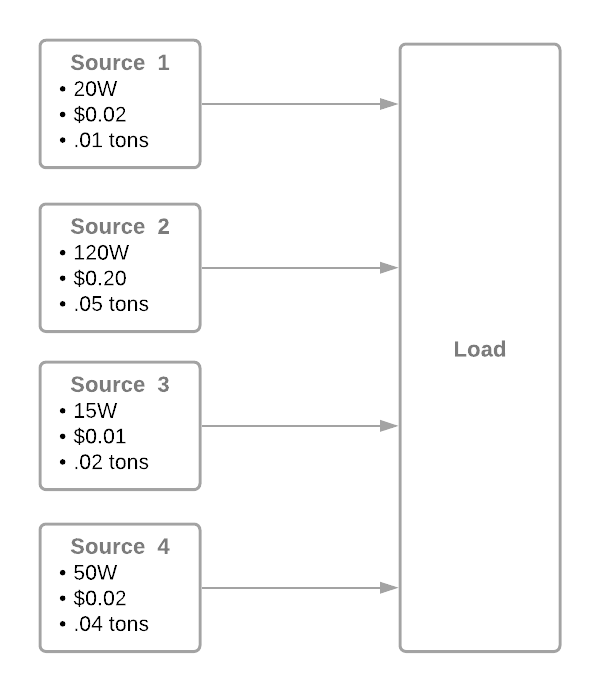
\includegraphics[height=6cm]{graphics/block_diagram.png}
    \end{center}
    \caption{Block Diagram}
    \label{fig:block}
    \end{figure}

    \subsection{Load Time Series}
    Here is a rough idea of what the load time series will look like. It is subject to change.
    \begin{figure}[h!]
        \begin{center}
            \includegraphics[height=6cm]{graphics/load_timeseries.png}
        \end{center}
        \caption{Load}
        \label{fig:load}
    \end{figure}

    \subsection{Load Time Series Generation}
    This time series was designed by deciding with the idea that the power is being sent to a residential area.  The usage would be low in the middle
    of the night and high when residents are home from work.  It would gradually
    increase/decrease throughout the other parts of the day.  The assumption
    is that a week days are being explored.

    To find the values, a range was given for each hour through out the day.
    A value for each hour within these ranges is randomly selected.  A set
    number of days can be produced.  In order to smooth out the curve an additional parameter was utilized to combine a set of days into a group and take the mean.  The purpose of this is to smooth out the curve into something that would look more realistic.

    \subsection{Source Chromosome Format}
    The chromosome format for each source is
    \[[cost, emission]\]

    \subsection{Gene Boundaries}
    Each gene has a power boundary corresponding to its potential source output.  The source can not output more than its limit.
    \begin{itemize}
        \item Source 1: [0, 20]
        \item Source 2: [0, 120]
        \item Source 3: [0, 15]
        \item Source 4: [0, 50]
    \end{itemize}

    \newpage
    \subsection{Economic Optimization}
    Economic optimization means that lower cost is better.  If the requirements can be met with lower cost this would be a beneficial economic adjustment.

    Economic boundary for fitness function:
    \begin{itemize}
        \item \(\$.15 \leq cost \leq \$6.55\)
        \begin{itemize}
            \item This range was chosen because the minimum is the least possible cost based on the power constraints and the max is the best possible cost plus a little extra due to the difficulty of finding the "best" solution in a GA.
        \end{itemize}
    \end{itemize}

    \subsection{Economic Fitness Boundaries}
    The economic fitness is ideally on a scale of 0 to 1, 0 being the most fit, but there will be some cases early on that goes off scale.
    \[W*\frac{cost-min}{max-min}\]
    
    \subsection{Environmental Optimization}
    Environmental optimization would imply that less emissions produced would be better for the environment.

    Environmental boundary for fitness function:
    \begin{itemize}
        \item \(.15  tons \leq emission \leq 3.75  tons\)
        \begin{itemize}
            \item Again, the lower bound is the least possible emission and the upper bound is the best plus a little extra.
        \end{itemize}
    \end{itemize}

    \subsection{Environmental Fitness Boundaries}
    The environmental fitness is ideally on a scale of 0 to 1, 0 being the most fit, but there will be some cases early on that goes off scale.
    After the emissions for the chromosome was calculated equation that was used to determine the fitness is:
    \[W*\frac{emssion-min}{max-min}\]

    \subsection{Boundary Function for Load}
        \begin{align*}
            15 \leq \sum_{i=1}^{n} P_i \leq 100
        \end{align*}

    \subsection{Population Size}
    \begin{itemize}
        \item Population size: 100    
    \end{itemize}
    \subsection{Mutation Rate}
    \begin{itemize}
        \item Mutation rate: .1
    \end{itemize}
    \subsection{Crossover Point}
    \begin{itemize}
        \item Crossover point: 2
    \end{itemize}
    \subsection{Stopping Condition}
    \begin{itemize}
        \item Stopping point: fitness \(\leq .08\)
    \end{itemize}

\setcounter{section}{2}
\clearpage
\section{Design Implementation}
    \begin{figure}[h!]
        \begin{center}
            \includegraphics[height=12cm]{graphics/GA.png}
        \end{center}                
    \end{figure}   
    \newpage
    \subsection{chromosome\_gen}
        \begin{figure}[h!]
            \begin{center}
                \includegraphics[height=8cm]{graphics/chromosome_gen.png}
            \end{center}                
        \end{figure}   
    \subsection{mutation}
    \begin{figure}[h!]
        \begin{center}
            \includegraphics[height=7cm]{graphics/mutation.png}
        \end{center}                
    \end{figure}  
    \newpage 
    \subsection{mutate}
    \begin{figure}[h!]
        \begin{center}
            \includegraphics[height=6cm]{graphics/mutate.png}
        \end{center}                
    \end{figure}   
    \subsection{crossover}
    \begin{figure}[h!]
        \begin{center}
            \includegraphics[height=9cm]{graphics/crossover.png}
        \end{center}                
    \end{figure}   
    \newpage
    \subsection{econ\_fitness}
    \begin{figure}[h!]
        \begin{center}
            \includegraphics[height=7cm]{graphics/econ_fitness.png}
        \end{center}                
    \end{figure}   
    \subsection{enviro\_fitness}
    \begin{figure}[h!]
        \begin{center}
            \includegraphics[height=7cm]{graphics/enviro_fitness.png}
        \end{center}                
    \end{figure}   
    \newpage
    \subsection{fitness}
    \begin{figure}[h!]
        \begin{center}
            \includegraphics[height=5cm]{graphics/fitness.png}
        \end{center}                
    \end{figure}   
    \subsection{Survival}
        \subsubsection{random\_selection}
        \begin{figure}[h!]
            \begin{center}
                \includegraphics[height=8cm]{graphics/random_selection.png}
            \end{center}                
        \end{figure}   
        \newpage
        \subsubsection{elitism}
        \begin{figure}[h!]
            \begin{center}
                \includegraphics[height=12cm]{graphics/elitism.png}
            \end{center}                
        \end{figure}   
    \newpage
    \subsection{stop\_condition}
    \begin{figure}[h!]
        \begin{center}
            \includegraphics[height=6cm]{graphics/stop_condition.png}
        \end{center}                
    \end{figure}   
    \subsection{store\_best}
    \begin{figure}[h!]
        \begin{center}
            \includegraphics[height=8cm]{graphics/store_best.png}
        \end{center}                
    \end{figure}  
    \newpage 
    \subsection{power\_plot}
    \begin{figure}[h!]
        \begin{center}
            \includegraphics[height=8cm]{graphics/power_plot.png}
        \end{center}                
    \end{figure}   
    \subsection{econ\_plot}
    \begin{figure}[h!]
        \begin{center}
            \includegraphics[height=6cm]{graphics/econ_plot.png}
        \end{center}                
    \end{figure} 
    \newpage  
    \subsection{enviro\_plot}
    \begin{figure}[h!]
        \begin{center}
            \includegraphics[height=6cm]{graphics/enviro_plot.png}
        \end{center}                
    \end{figure}   
    \subsection{calculation\_plot}
    \begin{figure}[h!]
        \begin{center}
            \includegraphics[height=6cm]{graphics/calculation_plot.png}
        \end{center}                
    \end{figure}  
    \newpage 
    \subsection{get\_data}
    \begin{figure}[h!]
        \begin{center}
            \includegraphics[height=10cm]{graphics/get_data.png}
        \end{center}                
    \end{figure}   
\newpage
\section{Additional Functions}
    \subsection{TimeSeries}
    \begin{figure}[h!]
        \begin{center}
            \includegraphics[height=12cm]{graphics/TimeSeries.png}
        \end{center}                
    \end{figure}   
    \newpage
    \subsection{check\_bounds}
    \begin{figure}[h!]
        \begin{center}
            \includegraphics[height=11cm]{graphics/check_bounds.png}
        \end{center}                
    \end{figure}   
    \newpage
    \subsection{find\_fitness}
    \begin{figure}[h!]
        \begin{center}
            \includegraphics[height=9cm]{graphics/find_fitness.png}
        \end{center}                
    \end{figure}   
    \subsection{mass\_mutate}
    \begin{figure}[h!]
        \begin{center}
            \includegraphics[height=6cm]{graphics/mass_mutate.png}
        \end{center}                
    \end{figure}   


\setcounter{section}{4}
\newpage
\section{Analysis}
    \subsection{Mutation \& Random Selection}
    \subsubsection{Excess Power}
        Excess power produced: 130W
            \begin{figure}[h!]
                \begin{center}
                    \includegraphics[height=6cm]{graphics/m_rs_power.png}
                \end{center}                
                \label{fig:MRSpower}
            \end{figure}        
        
        \subsubsection{Cost}
        Total cost for the day: \$54.37
            \begin{figure}[h!]
                \begin{center}
                    \includegraphics[height=6cm]{graphics/m_rs_econ.png}
                \end{center}                
                \label{fig:MRScost}
            \end{figure}
        \newpage    
        \subsubsection{Environmental Impact}
        Total emission for the day: 45.17 tons
            \begin{figure}[h!]
                \begin{center}
                    \includegraphics[height=6cm]{graphics/m_rs_enviro.png}
                \end{center}                
                \label{fig:MRSemissions}
            \end{figure}
        
        \subsubsection{Calculation Time}
            \begin{figure}[h!]
                \begin{center}
                    \includegraphics[height=6cm]{graphics/m_rs_calc.png}
                \end{center}                
                \label{fig:MRScalc}
            \end{figure}
    \newpage      
    \subsection{Mutation \& Elitism}
        \subsubsection{Excess Power}
        Excess power produced: 100W
            \begin{figure}[h!]
                \begin{center}
                    \includegraphics[height=6cm]{graphics/m_e_power.png}
                \end{center}                
                \label{fig:MEpower}
            \end{figure}        
        \subsubsection{Cost}
        Total cost for the day: \$60.33
            \begin{figure}[h!]
                \begin{center}
                    \includegraphics[height=6cm]{graphics/m_e_econ.png}
                \end{center}
                \label{fig:MEcost}
            \end{figure}
        \newpage    
        \subsubsection{Environmental Impact}
        Total emission for the day: 45.05 tons
            \begin{figure}[h!]
                \begin{center}
                    \includegraphics[height=6cm]{graphics/m_e_enviro.png}
                \end{center}                
                \label{fig:MEemissions}
            \end{figure}
        
        \subsubsection{Calculation Time}
            \begin{figure}[h!]
                \begin{center}
                    \includegraphics[height=6cm]{graphics/m_e_calc.png}
                \end{center}                
                \label{fig:MEcalc}
            \end{figure}
    \newpage    
    \subsection{Crossover \& Random Selection}
        \subsubsection{Excess Power}
            Excess power produced: 119W
            \begin{figure}[h!]
                \begin{center}
                    \includegraphics[height=6cm]{graphics/c_rs_power.png}
                \end{center}                
                \label{fig:CRSpower}
            \end{figure}        
        \subsubsection{Cost}
            Total cost for the day: \$52.48
            \begin{figure}[h!]
                \begin{center}
                    \includegraphics[height=6cm]{graphics/c_rs_econ.png}
                \end{center}                
                \label{fig:CRScost}
            \end{figure}
        \newpage   
        \subsubsection{Environmental Impact}
            Total emission for the day: 44.78 tons
            \begin{figure}[h!]
                \begin{center}
                    \includegraphics[height=6cm]{graphics/c_rs_enviro.png}
                \end{center}                
                \label{fig:CRSemissions}
            \end{figure}
        \subsubsection{Calculation Time}
            \begin{figure}[h!]
                \begin{center}
                    \includegraphics[height=6cm]{graphics/c_rs_calc.png}
                \end{center}                
                \label{fig:CRScalc}
            \end{figure}
    \newpage        
    \subsection{Crossover \& Elitism}
        \subsubsection{Excess Power}
            Excess power produced: 64W
            \begin{figure}[h!]
                \begin{center}
                    \includegraphics[height=6cm]{graphics/c_e_power.png}
                \end{center}
                \label{fig:CEpower}
            \end{figure}        
        \subsubsection{Cost}
            Total cost for the day: \$52.68
            \begin{figure}[h!]
                \begin{center}
                    \includegraphics[height=6cm]{graphics/c_e_econ.png}
                \end{center}
                \label{fig:CEcost}
            \end{figure}
        \newpage   
        \subsubsection{Environmental Impact}
            Total emission for the day: 43.79 tons
            \begin{figure}[h!]
                \begin{center}
                    \includegraphics[height=6cm]{graphics/c_e_enviro.png}
                \end{center}
                \label{fig:CEemissions}
            \end{figure}
        
        \subsubsection{Calculation Time}
            \begin{figure}[h!]
                \begin{center}
                    \includegraphics[height=6cm]{graphics/c_e_calc.png}
                \end{center}
                \label{fig:CEcalc}
            \end{figure}
            
    
    \newpage
    \subsection{Comparison}
    \subsubsection{Excess Power}
        It can be seen that the random mutations causes an increased amount of excess power that is produced due to its random nature.  Random selection also hinders the excess power even further when combined with random mutation. When mutation is paired with elitism, the results are slightly more efficient.  When crossover is combined with random selection, the results are similar to mutation due to its lack of diversity.  When crossover is combined with elitism, the best result are made due to only reproducing with the most elite chromosome for each generation.
    
    \subsubsection{Cost}
        The cost for each method is quite similar and behaves as you might expect.  The cost throughout the day typically follows the trend of the power output.
        the typical range for cost is \(\$50 \leq cost \leq \$65\)

    \subsubsection{Environmental Impact}
        The emissions also follows a similar trend to the power across all methods.  interestingly, the curve is typically a little wider than that of the power curve. Perhaps this is due to the defined weights. The range for emissions is typically \(40 \leq emissions \leq 48 \) tons

    \subsubsection{Calculation Time}
        The time it took to generate across all methods was quite predictable.  
        The main driving factor that hindered the calculation time was the survival method.  Random selection typically took longer than that of elitism.  Interestingly, the difference between mutation and crossover time was not that different as long as the crossover set received a good starting point. There are some cases where crossover is unsolvable due to lack of diversity.

\section{Recommendation}
    \subsection{Improvements}
    The initial chromosome generation could be optimized to use more realistic values and diverse.  Crossover benefits from larger data sets with more diversity as a starting point.  If the original chromosomes were intentionally more diverse there could be better results.  In the case that the good enough value is too low or the data set is not diverse enough the algorithm will run out of solutions to make it to the stopping condition.


    \subsection{Concerns to Be Addressed}
    One concern that is not addressed in this system is that there is no value for the maximum heat that the sources can produce before failure.  With this additional constraint there may be times were it would be more logical to increase cost and/or emissions in order to cool a source that has done a lot of work.  With the way the system is set up now, a source could go all day without any down time while another source doesn't do much.  The lack of this information could lead to catastrophic failure.

    Another concern is that there is no set limit how much extra power can be produced.  With no location for storage, the system could over load the load and could potentially cause fires or explosions depending on how much excess power is sent to the load.

\end{document}